\item {\bf Peeking Blackjack}

Now that we have gotten a bit of practice with general-purpose MDP algorithms,
let's use them to play (a modified version of) Blackjack. For this problem, you
will be creating an MDP to describe states, actions, and rewards in this game.

For our version of Blackjack, the deck can contain an arbitrary collection of
cards with different face values.  At the start of the game, the deck contains
the same number of each cards of each face value; we call this number the
`multiplicity'.  For example, a standard deck of 52 cards would have face values
$[1, 2, \ldots, 13]$ and multiplicity 4.  You could also have a deck with face
values $[1,5,20]$; if we used multiplicity 10 in this case, there would be 30
cards in total (10 each of 1s, 5s, and 20s). The deck is shuffled, meaning that\
each permutation of the cards is equally likely.

\begin{center}
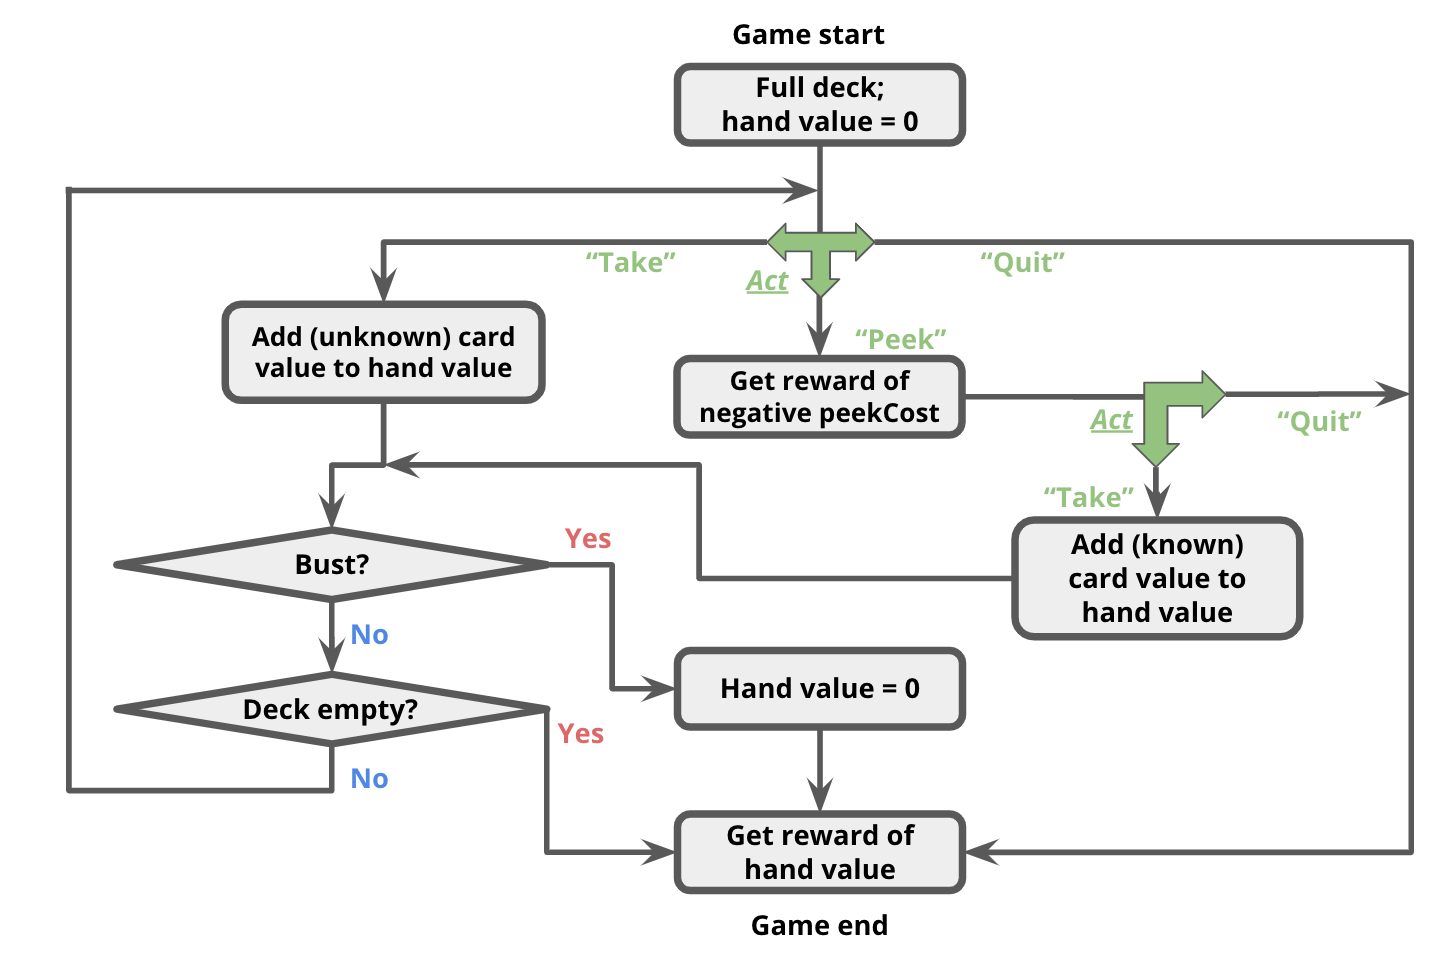
\includegraphics[width=0.5\textwidth]{03-peeking-blackjack/blackjack_rule.png}
\end{center}

The game occurs in a sequence of rounds. Each round, the player either (i) takes
the next card from the top of the deck (costing nothing), (ii) peeks at the top
card (costing |peekCost|, in which case the next round, that card will be
drawn), or (iii) quits the game. (Note: it is not possible to peek twice in a
row; if the player peeks twice in a row, then |succAndProbReward()| should
return |[]|.)

The game continues until one of the following conditions becomes true:
\begin{itemize}
  \item The player quits, in which case her reward is the sum of the face values
  of the cards in her hand.
  \item The player takes a card and "goes bust".  This means that the sum of the
  face values of the cards in her hand is strictly greater than the threshold
  specified at the start of the game.  If this happens, her reward is 0.
  \item The deck runs out of cards, in which case it is as if she quits, and she
  gets a reward which is the sum of the cards in her hand. {\em Make sure that
  if you take the last card and go bust, then the reward becomes 0 not the sum
  of values of cards.}
\end{itemize}

In this problem, your state $s$ will be represented as a 3-element tuple:
\begin{lstlisting}  
(totalCardValueInHand, nextCardIndexIfPeeked, deckCardCounts)
\end{lstlisting}

As an example, assume the deck has card values $[1, 2, 3]$ with multiplicity 1,
and the threshold is 4. Initially, the player has no cards, so her total is 0;
this corresponds to state |(0, None, (1, 1, 1))|. At this point, she can take,
peek, or quit.
\begin{itemize}
  \item If she takes, the three possible successor states (each of which has
  equal probability of $1/3$) are:
\begin{lstlisting}
(1, None, (0, 1, 1))
(2, None, (1, 0, 1))
(3, None, (1, 1, 0))
\end{lstlisting}
  She will receive a reward of 0 for reaching any of these states.  (Remember,
  even though she now has a card in her hand for which she may receive a reward
  at the end of the game, the reward is not actually granted until the game
  ends.)
  \item If she peeks, the three possible successor states are:
\begin{lstlisting}
(0, 0, (1, 1, 1))
(0, 1, (1, 1, 1))
(0, 2, (1, 1, 1))
\end{lstlisting}
  She will receive (immediate) reward |-peekCost| for reaching any of these
  states. Things to remember about the states after a peek action:
  \begin{itemize}
    \item From |(0, 0, (1, 1, 1))|, taking a card will lead to the state |(1, None, (0, 1, 1))| deterministically.
    \item The second element of the state tuple is not the face value of the
    card that will be drawn next, but the index into the deck (the third element
    of the state tuple) of the card that will be drawn next.  In other words,
    the second element will always be between 0 and |len(deckCardCounts)-1|,
    inclusive.
  \end{itemize}
  \item If she quits, then the resulting state will be |(0, None, None)|.
  (Remember that setting the deck to |None| signifies the end of the game.)
\end{itemize}

As another example, let's say the player's current state is |(3, None, (1, 1, 0))|, and the threshold remains 4.
\begin{itemize}
  \item If she quits, the successor state will be |(3, None, None)|.
  \item If she takes, the successor states are |(3 + 1, None, (0, 1, 0))| or |(3 + 2, None, None)|.
\end{itemize}

Note that in the second successor state, the deck is set to |None| to signify
the game ended with a bust. You should also set the deck to |None| if the deck
runs out of cards.

\begin{enumerate}

  \item \points{3a}
Implement the game of Blackjack as an MDP by filling out the
|succAndProbReward()| function of class |BlackjackMDP|.


\end{enumerate}
